\documentclass[11pt,fleqn]{article}
\usepackage{../cs188,latexsym,epsf, amsmath,amsfonts,graphicx,url,multicol}
\usepackage{caption}
\usepackage{subcaption}
\lecture{1}
\def\title{Note \the\lecturenumber}
\begin{document}
\maketitle


\iffalse
\documentclass[11pt,fleqn]{article}
\usepackage{latexsym,epsf,amsmath,amsfonts,graphicx,url}

\title{Note 1}

\newcommand{\F}{\mathbb{F}}
\newcommand{\Z}{\mathbb{Z}}
\newcommand{\Q}{\mathbb{Q}}
\newcommand{\R}{\mathbb{R}}
\newcommand{\C}{\mathbb{C}}

\begin{document}

\maketitle
\fi

\section*{Agents}

In artificial intelligence, the central problem at hand is that of the creation of a rational \textbf{agent}, an entity that has goals or preferences and tries to perform a series of \textbf{actions} that yield the best/optimal expected outcome given these goals. Rational agents exist in an \textbf{environment}, which is specific to the given instantiation of the agent. As a very simple example, the environment for a checkers agent is the virtual checkers board on which it plays against opponents, where piece moves are actions. Together, an environment and the agents that reside within it create a \textbf{world}. 

A \textbf{reflex agent} is one that doesn't think about the consequences of its actions, but rather selects an action based solely on the current state of the world. These agents are typically outperformed by \textbf{planning agents}, which maintain a model of the world and use this model to simulate performing various actions. Then, the agent can determine hypothesized consequences of the actions and can select the best one. This is simulated "intelligence" in the sense that it's exactly what humans do when trying to determine the best possible move in any situation - thinking ahead.

\section*{State Spaces and Search Problems}
In order to create a rational planning agent, we need a way to mathematically express the given environment in which the agent will exist. To do this, we must formally express a \textbf{search problem} - given our agent's current \textbf{state} (its configuration within its environment), how can we arrive at a new state that satisfies its goals in the best possible way? Formulating such a problem requires four things:
	\begin{itemize}
		\item A \textbf{state space} - The set of all possible states that are possible in your given world
		\item A \textbf{successor function} - A function that takes in a state and an action and computes the cost of performing that action as well as the \textbf{successor state}, the state the world would be in if the given agent performed that action
		\item A \textbf{start state} - The state in which an agent exists initially
		\item A \textbf{goal test} - A function that takes a state as input, and determines whether it is a goal state
	\end{itemize}
Fundamentally, a search problem is solved by first considering the start state, then exploring the state space using the successor function, iteratively computing successors of various states until we arrive at a goal state, at which point we will have determined a path from the start state to the goal state (typically called a \textbf{plan}). The order in which states are considered is determined using a predetermined \textbf{strategy}. We'll cover types of strategies and their usefulness shortly.

Before we continue with how to solve search problems, it's important to note the difference between a \textbf{world state}, and a \textbf{search state}. A world state contains all information about a given state, whereas a search state contains only the information about the world that's necessary for planning (primarily for space effiency reasons). To illustrate these concepts, we'll introduce the hallmark motivating example of this course - Pacman. The game of Pacman is simple: Pacman must navigate a maze and eat all the (small) food pellets in the maze without being eaten by the malicious patrolling ghosts. If Pacman eats one of the (large) power pellets, he becomes ghost-immune for a set period of time and gains the ability to eat ghosts for points. 

\begin{center}
	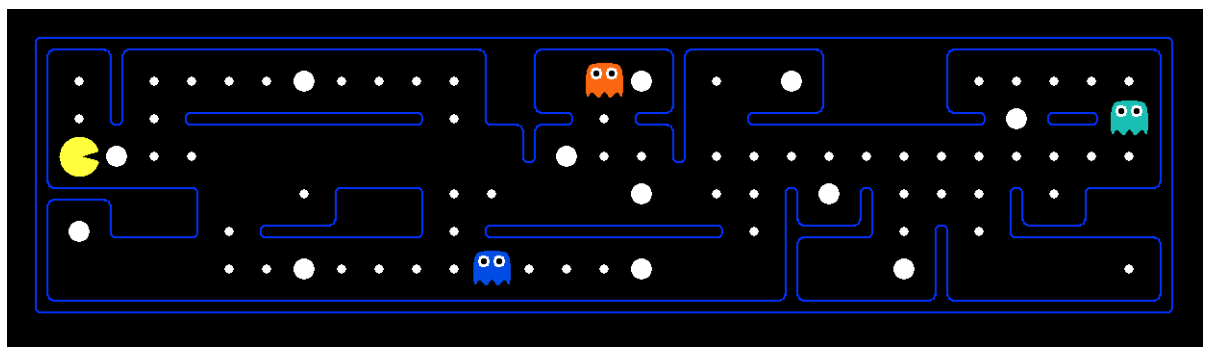
\includegraphics[width=16.5cm]{img/pacman_example}
\end{center}

Let's consider a variation of the game in which the maze contains only Pacman and food pellets. We can pose two distinct search problems in this scenario: pathing and eat-all-dots. Pathing attempts to solve the problem of getting from position $(x_1, y_1)$ to position $(x_2, y_2)$ in the maze optimally, while eat all dots attempts to solve the problem of consuming all food pellets in the maze in the shortest time possible. Below, the states, actions, successor function, and goal test for both problems are listed:
\begin{multicols}{2}
\begin{itemize}
\item{\textbf{Pathing}}
	\begin{itemize}
		\item States: (x,y) locations
		\item Actions: North, South, East, West
		\item Successor: Update location only
		\item Goal test: Is (x,y)=END?
	\end{itemize}
\item{\textbf{Eat-all-dots}}
	\begin{itemize}
		\item States: {(x,y) location, dot booleans}
		\item Actions: North, South, East, West
		\item Successor: Update location and booleans
		\item Goal test: Are all dot booleans false?
	\end{itemize}
\end{itemize}
\end{multicols}

Note that for pathing, states contain less information than states for eat-all-dots, because for eat-all-dots we must maintain an array of booleans corresponding to each food pellet and whether or not it's been eaten in the given state. A world state may contain more information still, potentially encoding information about  things like total distance traveled by Pacman or all positions visited by Pacman on top of its current (x,y) location and dot booleans.

\subsection*{State Space Size} 
An important question that often comes up while estimating the computational runtime of solving a search problem is the size of the state space. This is done almost exclusively with the \textbf{fundamental counting principle}, which states that if there are $n$ variable objects in a given world which can take on $x_1$, $x_2$, ..., $x_n$ different values respectively, then the total number of states is $x_1 \cdot x_2 \cdot ... \cdot x_n$. Let's use Pacman to show this concept by example:
	\begin{center}
		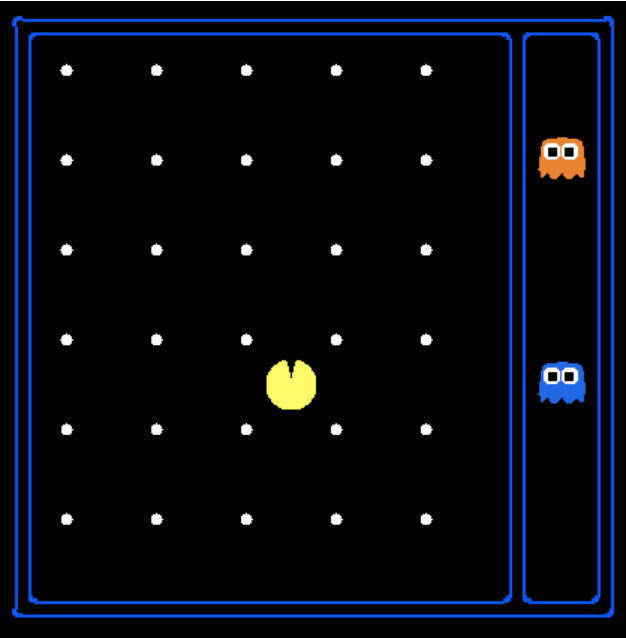
\includegraphics[height=6cm,width=6cm]{img/state_space_size}
	\end{center}
Let's say that the variable objects and their corresponding number of possiblilites are as follows:
	\begin{itemize}
		\item \textit{Pacman positions} - Pacman can be in 120 distinct $(x,y)$ positions, and there is only one Pacman
		\item \textit{Pacman Direction} - this can be North, South, East, or West, for a total of 4 possibilities
		\item \textit{Ghost positions} - There are two ghosts, each of which can be in 12 distinct $(x,y)$ positions
		\item \textit{Food pellet configurations} - There are 30 food pellets, each of which can be eaten or not eaten
	\end{itemize}
Using the fundamental counting principle, we have $120$ positions for Pacman, $4$ directions Pacman can be facing, $12 \cdot 12$ ghost configurations (12 for each ghost), and $2 \cdot 2 \cdot ... \cdot 2 = 2^{30}$ food pellet configurations (each of 30 food pellets has two possible values - eaten or not eaten). This gives us a total state space size of $\boxed{120 \cdot 4 \cdot 12^2 \cdot 2^{30}}$.

\subsection*{State Space Graphs and Search Trees}
Now that we've established the idea of a state space and the four components necessary to completely define one, we're almost ready to begin solving search problems. The final piece of the puzzle is that of state space graphs and search trees.

Recall that a graph is defined by a set of nodes and a set of edges connecting various pairs of nodes. These edges may also have weights associated with them. A \textbf{state space graph} is constructed with states representing nodes, with directed edges existing from a state to its successors. These edges represent actions, and any associated weights represent the cost of performing the corresponding action. Typically, state space graphs are much too large to store in memory (even our simple Pacman example from above has $\approx 10^{13}$ possible states, yikes!), but they're good to keep in mind conceptually while solving problems. It's also important to note that in a state space graph, each state is represented exactly once - there's simply no need to represent a state multiple times, and knowing this helps quite a bit when trying to reason about search problems.

Unlike state space graphs, our next structure of interest, \textbf{search trees}, have no such restriction on the number of times a state can appear. This is because though search trees are also a class of graph with states as nodes and actions as edges between states, each state/node encodes not just the state itself, but the entire path (or \textbf{plan}) from the start state to the given state in the state space graph. Observe the state space graph and corresponding search tree below:
	\begin{center}
		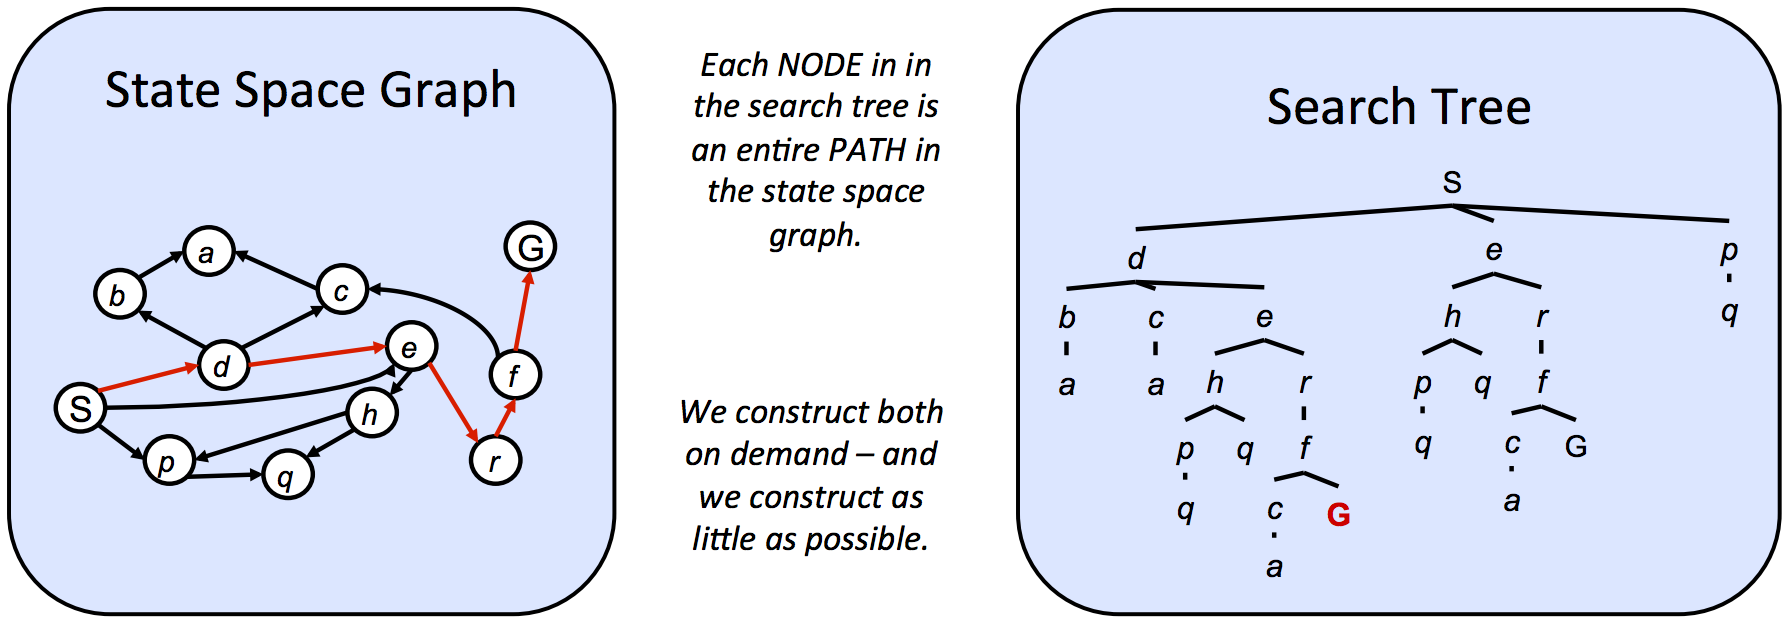
\includegraphics[width=15cm,height=6cm]{img/graph_and_tree}
	\end{center}
The highlighted path (S $\rightarrow$ d $\rightarrow$ e $\rightarrow$ r $\rightarrow$ f $\rightarrow$ G) in the given state space graph is represented in the corresponding search tree by following the path in the tree from the start state $S$ to the highlighted goal state $G$. Similarly, each and every path from the start node to any other node is represented in the search tree by a path from the root $S$ to some descendant of the root corresponding to the other node. Since there often exist multiple ways to get from one state to another, states tend to show up multiple times in search trees. As a result, search trees are greater than or equal to their corresponding state space graph in size. 

We've already determined that state space graphs themselves can be enormous in size even for simple problems, and so the question arises - how can we perform useful computation on these structures if they're too big to represent in memory? The answer lies in successor functions - we only store states we're immediately working with, and compute new ones on-demand using the corresponding successor function. Typically, search problems are solved using search trees, where we very carefully store a select few nodes to observe at a time, iteratively replacing nodes with their successors until we arrive at a goal state. There exist various methods by which to decide the order in which to conduct this iterative replacement of search tree nodes, and we'll present these methods now.

\section*{Uninformed Search}
The standard protocol for finding a plan to get from the start state to a goal state is to maintain an outer \textbf{fringe} of partial plans derived from the search tree. We continually \textbf{expand} our fringe by removing a node (which is selected using our given \textbf{strategy}) corresponding to a partial plan from the fringe, and replacing it on the fringe with all its children. Removing and replacing an element on the fringe with its children corresponds to discarding a single length $n$ plan and bringing all length $(n+1)$ plans that stem from it into consideration. We continue this until eventually removing a goal state off the fringe, at which point we conclude the partial plan corresponding to the removed goal state is in fact a path to get from the start state to the goal state. This procedure we have just outlined is known as \textbf{tree search}, and the pseudocode for it is presented below:
	\begin{center}
		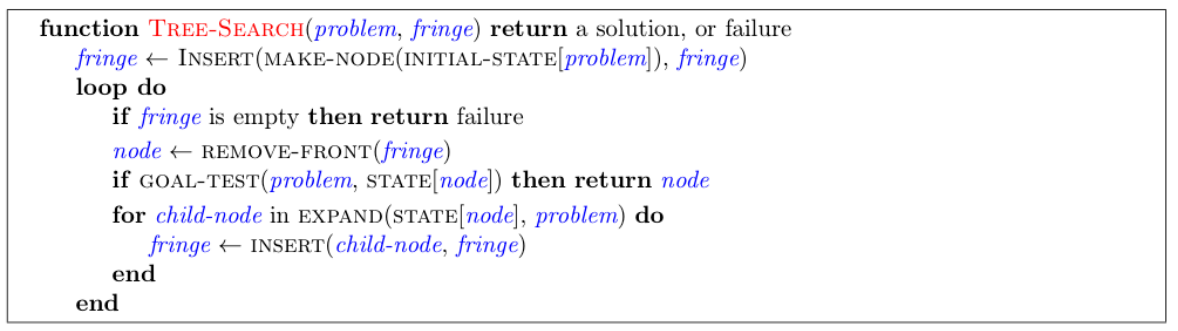
\includegraphics[height=5cm,width=15cm]{img/tree_search_pseudocode}
	\end{center}

When we have no knowledge of the location of goal states in our search tree, we are forced to select our strategy for tree search from one of the techniques that falls under the umbrella of \textbf{uninformed search}. We'll now cover three such strategies in succession: \textbf{depth-first search}, \textbf{breadth-first search}, and \textbf{uniform cost search}. Along with each strategy, some rudimentary properties of the strategy are presented as well, in terms of the following:
	\begin{itemize}
		\item The \textbf{completeness} of each search strategy - if there exists a solution to the search problem, is the strategy guaranteed to find it given infinite computational resources?
		\item The \textbf{optimality} of each search strategy - is the strategy guaranteed to find the lowest cost path to a goal state?
		\item The \textbf{branching factor} $b$ - The increase in the number of nodes on the fringe each time a fringe node is dequeued and replaced with its children is $O(b)$. At depth $k$ in the search tree, there exists $O(b^k)$ nodes.
		\item The maximum depth $m$.
		\item The depth of the shallowest solution $s$.
	\end{itemize}

\subsection*{Depth-First Search}
\begin{itemize}
\item \textit{Description} - Depth-first search (DFS) is a strategy for exploration that always selects the \textit{deepest} fringe node from the start node for expansion. 
\item \textit{Fringe representation} - Removing the deepest node and replacing it on the fringe with its children necessarily means the children are now the new deepest nodes - their depth is one greater than the depth of the previous deepest node. This implies that to implement DFS, we require a structure that always gives the most recently added objects highest priority. A last-in, first-out (LIFO) stack does exactly this, and is what is traditionally used to represent the fringe when implementing DFS.
\begin{center}
	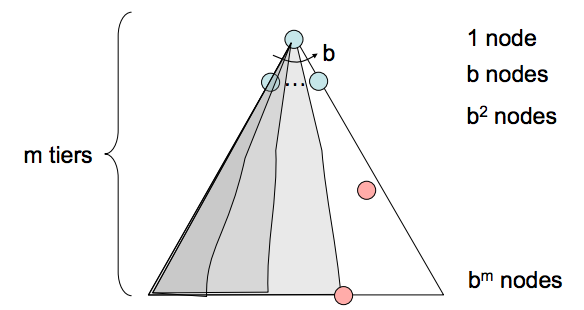
\includegraphics[width=7cm, height=4cm]{img/dfs}
\end{center}
\item \textit{Completeness} - Depth-first search is not complete. If there exists cycles in the state space graph, this inevitably means that the corresponding search tree will be infinite in depth. Hence, there exists the possibility that DFS will faithfully yet tragically get "stuck" searching for the deepest node in an infinite-sized search tree, doomed to never find a solution.
\item \textit{Optimality} - Depth-first search simply finds the "leftmost" solution in the search tree without regard for path costs, and so is not optimal.
\item \textit{Time Complexity} - In the worst case, depth first search may end up exploring the entire search tree. Hence, given a tree with maximum depth $m$, the runtime of DFS is $O(b^m)$.
\item \textit{Space Complexity} - In the worst case, DFS maintains $b$ nodes at each of $m$ depth levels on the fringe. This is a simple consequence of the fact that once $b$ children of some parent are enqueued, the nature of DFS allows only one of the subtrees of any of these children to be explored at any given point in time. Hence, the space complexity of BFS is $O(bm)$.
\end{itemize}

\subsection*{Breadth-First Search}
\begin{itemize}
\item \textit{Description} - Breadth-first search is a strategy for exploration that always selects the \textit{shallowest} fringe node from the start node for expansion. 
\item \textit{Fringe representation} - If we want to visit shallower nodes before deeper nodes, we must visit nodes in their order of insertion. Hence, we desire a structure that outputs the oldest enqueued object to represent our fringe. For this, BFS uses a first-in, first-out (FIFO) queue, which does exactly this.
\begin{center}
	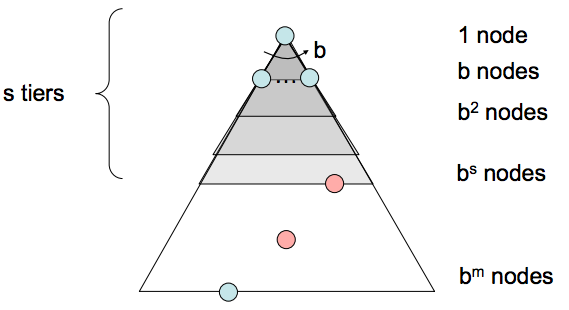
\includegraphics[width=7cm, height=4cm]{img/bfs}
\end{center}
\item \textit{Completeness} - If a solution exists, then the depth of the shallowest node $s$ must be finite, so BFS must eventually search this depth. Hence, it's complete.
\item \textit{Optimality} - BFS is generally not optimal because it simply does not take costs into consideration when determining which node to replace on the fringe. The special case where BFS is guaranteed to be optimal is if all edge costs are equivalent, because this reduces BFS to a special case of uniform cost search, which is discussed below.
\item \textit{Time Complexity} - We must search $1 + b + b^2 + ... + b^s$ nodes in the worst case, since we go through all nodes at every depth from 1 to $s$. Hence, the time complexity is $O(b^s)$.
\item \textit{Space Complexity} - The fringe, in the worst case, contains all the nodes in the level corresponding to the shallowest solution. Since the shallowest solution is located at depth $s$, there are $O(b^s)$ nodes at this depth.
\end{itemize}

\subsection*{Uniform Cost Search}
\begin{itemize}
\item \textit{Description} - Uniform cost search (UCS), our last strategy, is a strategy for exploration that always selects the \textit{lowest cost} fringe node from the start node for expansion.
\item \textit{Fringe representation} - To represent the fringe for UCS, the choice is usually a heap-based priority queue, where the weight for a given enqueued node is the path cost from the start node to that node. Intuitively, a priority queue constructed in this manner simply reshuffles itself to maintain the desired ordering by path cost as we remove the current minimum cost path and replace it with its children.
\begin{center}
	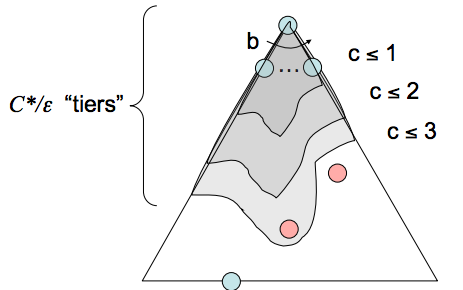
\includegraphics[width=7cm, height=4cm]{img/ucs}
\end{center}
\item \textit{Completeness} - Uniform cost search is complete. If a goal state exists, it must have some finite length shortest path; hence, UCS must eventually find this shortest length path.
\item \textit{Optimality} - UCS is also optimal if we assume all edge costs are nonnegative. By construction, since we explore nodes in order of increasing path cost, we're guaranteed to find the lowest-cost path to a goal state. Note that having negative edge costs in our graph can make nodes on a path have decreasing length, ruining our guarantee of optimality.
\item \textit{Time Complexity} - Let us define the optimal past cost as $C^*$ and the minimal cost between two nodes in the state space graph as $\epsilon$. Then, we must roughly explore all nodes at depths ranging from 1 to $C^*/\epsilon$, leading to an runtime of $O(b^{C^*/\epsilon})$.
\item \textit{Space Complexity} - Roughly, the fringe will contain all nodes at the level of the cheapest solution, so the space complexity of UCS is estimated as $O(b^{C^*/\epsilon})$.
\end{itemize}

As a parting note about uninformed search, it's critical to note that the three strategies outlined above are fundamentally the same - differing only in expansion strategy, with their similarities being captured by the tree search pseudocode presented above.

\section*{Informed Search}
Uniform cost search is good because it's both complete and optimal, but it can be fairly slow because it expands in every direction from the start state while searching for a goal. If we have some notion of the direction in which we should focus our search, we can significantly improve performance and "hone in" on a goal much more quickly. This is exactly the focus of \textbf{informed search}.

\subsection*{Heuristics}
\textbf{Heuristics} are the driving force that allow estimation of distance to goal states - they're functions that take in a state as input and output a corresponding estimate. Heuristic functions are typically solutions to \textbf{relaxed problems}, and the computation performed by such a function is specific to the search problem being solved. Turning to our Pacman example, let's consider the pathing problem described earlier. A common heuristic that's used to solve this problem is the \textbf{Manhattan distance}, which for two points $(x_1, y_1)$ and $(x_2, y_2)$ is defined as follows: $$Manhattan(x_1, y_1, x_2, y_2) = |x_1 - x_2| + |y_1 - y_2|$$
\begin{center}
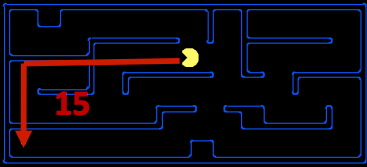
\includegraphics{img/manhattan}
\end{center}
The above visualization shows the relaxed problem that the Manhattan distance helps solve - assuming Pacman desires to get to the bottom left corner of the maze, it computes the distance from Pacman's current location to Pacman's desired location \textit{assuming a lack of walls in the maze}. This distance is the \textit{exact} goal distance in the relaxed search problem, and correspondingly is the \textit{estimated} goal distance in the actual search problem. With heuristics, it becomes very easy to implement logic in our agent that enables them to "prefer" expanding states that are estimated to be closer to goal states when deciding which action to perform. This concept of preference is very powerful, and is utilized by the following two search algorithms that implement heuristic functions: greedy search and A*.

\subsection*{Greedy Search}
\begin{itemize}
\item \textit{Description} - Greedy search is a strategy for exploration that always selects the fringe node with the \textit{lowest heuristic value} for expansion, which corresponds to the state it believes is nearest to a goal.
\item \textit{Fringe representation} - Greedy search operates identically to UCS, with a priority queue fringe representation. The difference is that instead of using \textit{computed backward cost} to assign priority, greedy search uses \textit{estimated forward cost} in the form of heuristic values.
\item \textit{Completeness and Optimality} - Greedy search is not guaranteed to find a goal state if one exists, nor is it optimal, particularly in cases where a very bad heuristic function is selected. It generally acts fairly unpredictably from scenario to scenario, and can range from going straight to a goal state to acting like a badly-guided DFS and exploring all the wrong areas.
\end{itemize}

\begin{center}
\begin{figure}[!h]
\centering
\begin{subfigure}{.5\textwidth}
  \centering
  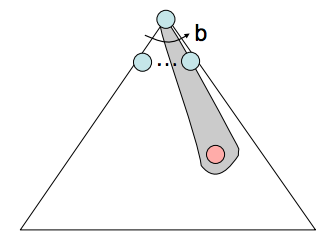
\includegraphics[width=.4\linewidth]{img/good_greedy}
  \caption{Greedy search on a good day :)}
  \label{fig:sub1}
\end{subfigure}%
\begin{subfigure}{.5\textwidth}
  \centering
  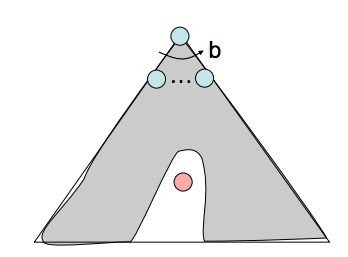
\includegraphics[width=.4\linewidth]{img/bad_greedy}
  \caption{Greedy search on a bad day :(}
  \label{fig:sub2}
\end{subfigure}
\label{fig:test}
\end{figure}
\end{center}


\subsection*{A* Search}
\begin{itemize}
\item \textit{Description} - A* search is a strategy for exploration that always selects the fringe node with the \textit{lowest estimated total cost} for expansion, where total cost is the entire cost from the start node to the goal node.
\item \textit{Fringe representation} - Just like greedy search and UCS, A* search also uses a priority queue to represent its fringe. Again, the only difference is the method of priority selection. A* combines the total backward cost used by UCS with the estimated forward cost used by greedy search by adding these two values, effectively yielding an \textit{estimated total cost} from start to goal. Given that we want to minimize the total cost from start to goal, this is an excellent choice.
\item \textit{Completeness and Optimality} - A* search is both complete and optimal, given an appropriate heuristic (which we'll cover in a minute). It's a combination of the good from all the other search strategies we've covered so far, incorporating the generally high speed of greedy search with the optimality and completeness of UCS!
\end{itemize}

\subsection*{Admissibility and Consistency}
Now that we've discussed heuristics and how they are applied in both greedy and A* search, let's spend some time discussing what constitutes a good heuristic. To do so, let's first reformulate the methods used for determining priority queue ordering in UCS, greedy search, and A* search slightly more mathematically, with the following definitions:
\begin{itemize}
\item $g(n)$ - The function representing total backwards cost computed by UCS to determine expansion order.
\item $h(n)$ - The \textit{heuristic value} function, used by greedy search to determine expansion order.
\item $f(n)$ - The function used by A* search to determine expansion order. $f(n) = g(n) + h(n)$.
\end{itemize}
Before attacking the question of what constitutes a "good" heuristic, we must first answer the question of whether A* maintains its properties of completeness and optimality regardless of the heuristic function we use. Indeed, it's very easy to find heuristics that break these two coveted properties. As an example, consider the heuristic function $h(n) = 1 - g(n)$. Regardless of the search problem, using this heuristic yields 
\begin{eqnarray*}
	f(n) &=& g(n) + h(n) \\
	&=& g(n) + (1 - g(n)) \\
	&=& 1
\end{eqnarray*}
Hence, such a heuristic reduces A* search to BFS, where all edge costs are equivalent. As we've already shown, BFS is not guaranteed to be optimal.

The condition required for optimality when using A* tree search is known as \textbf{admissibility}. The admissibility constraint states that the value estimated by an admissible heuristic is neither negative nor an overestimate. Defining $h^*(n)$ as the true optimal cost to reach a goal state from a given node $n$, we can formulate the admissibility constraint mathematically as follows: 

$$\forall{n}, \:\: 0 \leq h(n) \leq h^*(n)$$
\textbf{Theorem.} For a given search problem, if the admissibility constraint is satisfied by a heuristic function $h$, using A* tree search with $h$ on that search problem will yield an optimal solution.

\textit{Proof.} Assume two reachable goal states are located in the search tree for a given search problem, an optimal goal $A$ and a suboptimal goal $B$. Some ancestor $n$ of $A$ (including perhaps $A$ itself) must currently be on the fringe, since $A$ is reachable from the start state. We claim $n$ will be selected for expansion before $B$, using the following three statements:
	\begin{enumerate}
		\item $f(n) \leq f(A)$, because $n$ is an ancestor of $A$ and so is expanded before $A$.
		\item $g(A) < g(B)$. Because $A$ is given to be optimal and $B$ is given to be suboptimal, we can conclude that $A$ has a lower backwards cost to the start state than $B$.
		\item $h(A) = h(B) = 0$, because we are given that our heuristic satisfies the admissibility constraint. Since both $A$ and $B$ are both goal states, the true optimal cost to a goal state from $A$ or $B$ is simply $h^*(n) = 0$; hence $0 \leq h(n) \leq 0$.
	\end{enumerate}
We can combine statements 2. and 3. to conclude that $f(A) < f(B)$ as follows:
$$f(A) = g(A) + h(A) = g(A) < g(B) = g(B) + h(B) = f(B)$$
A simple consequence of combining the above derived inequality with statement 1. is the following:
 $$f(n) \leq f(A) \wedge f(A) < f(B) \Longrightarrow f(n) < f(B)$$
 Hence, we can conclude that $n$ is expanded before $B$. Because we have proven this for arbitrary $n$, we can conclude that \textit{all} ancestors of $A$ (including $A$ itself) expand before $B$. $\Box$

One problem we found above with tree search was that in some cases it could fail to ever find a solution, getting stuck searching the same cycle in the state space graph infinitely. Even in situations where our search technique doesn't involve such an infinite loop, it's often the case that we revisit the same node multiple times because there's multiple ways to get to that same node. This leads to exponentially more work, and the natural solution is to simply keep track of which states you've already expanded, and never expand them again. More explicitly, maintain a "closed" set of expanded nodes while utilizing your search method of choice. Then, ensure that each node isn't already in the set before expansion and add it to the set after expansion if it's not. Tree search with this added optimization is known as \textbf{graph search}, and the pseudocode for it is presented below:
\begin{center}
	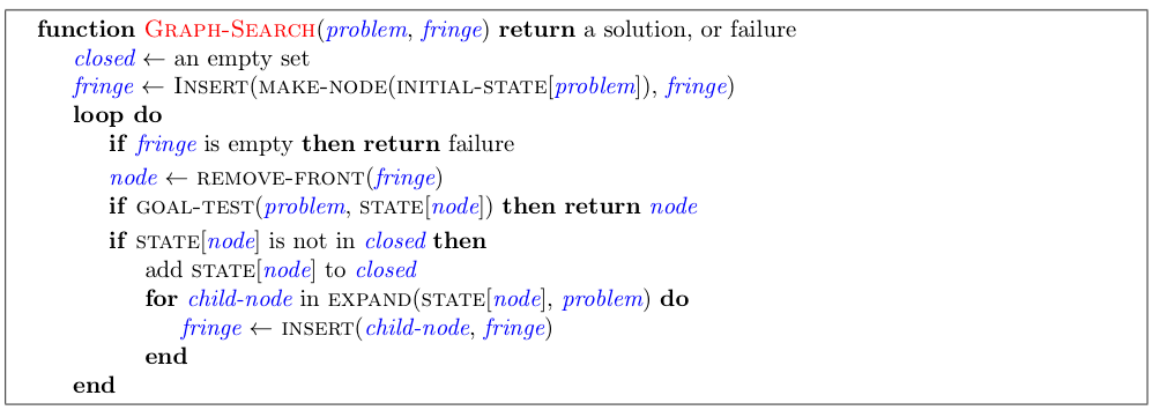
\includegraphics[height=6cm,width=15cm]{img/graph_search_pseudocode}
\end{center}
Note that in implementation, it's critically important to store the closed set as a disjoint set and not a list. Storing it as a list requires costs $O(n)$ operations to check for membership, which eliminates the performance improvement graph search is intended to provide. An additional caveat of graph search is that it tends to ruin the optimality of A*, even under admissible heuristics. Consider the following simple state space graph and corresponding search tree, annotated with weights and heuristic values:
\begin{center}
	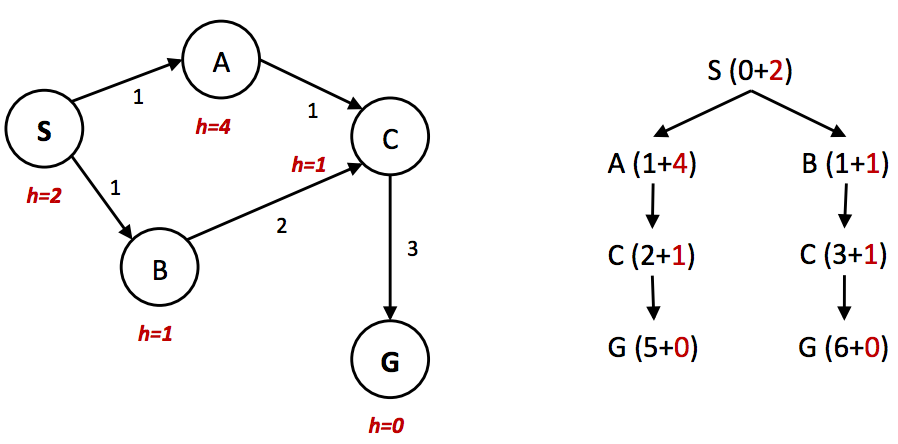
\includegraphics[height=7cm]{img/bad_graph_search}
\end{center}
In the above example, it's clear that the optimal route is to follow $S \rightarrow A \rightarrow C \rightarrow G$, yielding a total path cost of $1 + 1 + 2 = 5$. The only other path to the goal, $S \rightarrow B \rightarrow C \rightarrow G$ has a path cost of $1 + 2 + 2 = 6$. However, because the heuristic value of node $A$ is so much larger than the heuristic value of node $B$, node $C$ is first expanded along the second, suboptimal path as a child of node $B$. It's then placed into the "closed" set, and so A* graph search fails to reexpand it when it visits it as a child of $A$, so it never finds the optimal solution. Hence, to maintain completeness and optimality under A* graph search, we need an even stronger property than admissibility, \textbf{consistency}. The central idea of consistency is that we enforce not only that a heuristic underestimates the \textit{total} distance to a goal from any given node, but also the cost/weight of each edge in the graph. The cost of an edge as measured by the heurstic function is simply the difference in heuristic values for two connected nodes. Mathematically, the consistency constraint can be expressed as follows:
$$\forall A,C \quad h(A) - h(C) \leq cost(A,C)$$
\textbf{Theorem.} For a given search problem, if the consistency constraint is satisfied by a heuristic function $h$, using A* graph search with $h$ on that search problem will yield an optimal solution.

\textit{Proof.} In order to prove the above theorem, we first prove that when running A* graph search with a consistent heuristic, whenever we remove a node for expansion, we've found the optimal path to that node.

Using the consistency constraint, we can show that the values of $f(n)$ for nodes along any plan are nondecreasing. Define two nodes, $n$ and $n'$, where $n'$ is a successor of $n$. Then:
	\begin{eqnarray*}
		f(n') &=& g(n') + h(n') \\
		&=& g(n) + cost(n, n') + h(n') \\
		&\geq& g(n) + h(n) \\
		&=& f(n)
	\end{eqnarray*}
If for every parent-child pair $(n', n)$ along a path, $f(n') \geq f(n)$, then it must be the case that the values of $f(n)$ are nondecreasing along that path. With this information, we can now show that whenever a node $n$ is removed for expansion, its optimal path has been found. Assume towards a contradiction that this is false - that when $n$ is removed from the fringe, the path found to $n$ is suboptimal. This means that there must be some ancestor of $n$, $n''$, on the fringe that was never expanded but is on the optimal path to $n$. Contradiction! We've already shown that values of $f$ along a path are nondecreasing, and so $n''$ would have been removed for expansion before $n$. 

All we have left to show to complete our proof is that an optimal goal $A$ will always be removed for expansion and returned before any suboptimal goal $B$. This is trivial, since $h(A) = h(B) = 0$, so $$f(A) = g(A) < g(B) = f(B)$$just as in our proof of optimality of A* tree search under the admissibility constraint. Hence, we can conclude that A* graph search is optimal under a consistent heuristic. $\Box$

A couple of important highlights from the discussion above before we proceed: for heuristics that are either admissible/consistent to be valid, it must by definition be the case that $h(G) = 0$ for any goal state $G$. Additionally, consistency is not just a stronger constraint than admissibility, consistency \textit{implies} admissibility. This stems simply from the fact that if no edge costs are overestimates (as guaranteed by consistency), the total estimated cost from any node to a goal will also fail to be an overestimate.

Consider the following three-node network for an example of an admissible but inconsistent heuristic:
	\begin{center}
		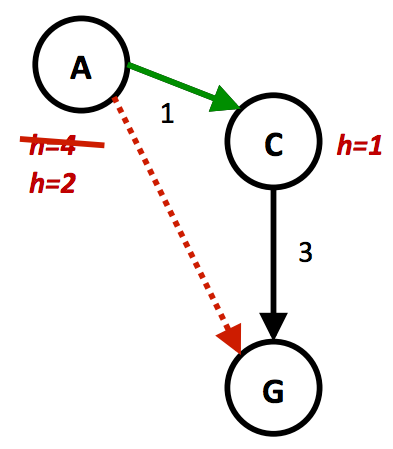
\includegraphics[height=4.9cm]{img/consistent_heuristic}
	\end{center}
The red dotted line corresponds to the total estimated goal distance. If $h(A) = 4$, then the heuristic is admissible, as the distance from $A$ to the goal is $4 \geq h(A)$, and same for $h(C) = 1 \leq 3$. However, the heuristic cost from $A$ to $C$ is $h(A) - h(C) = 4 - 1 = 3$. Our heuristic estimates the cost of the edge between $A$ and $C$ to be $3$ while the true value is $cost(A,C) = 1$, a smaller value. Since $h(A) - h(C) \nleq cost(A,C)$, this heuristic is not consistent. Running the same computation for $h(A) = 2$, however, yields $h(A) - h(C) = 2 - 1 = 1 \leq cost(A,C)$. Thus, using $h(A) = 2$ makes our heuristic consistent.

\subsection*{Dominance}
Now that we've established the properties of admissibility and consistency and their roles in maintaining the optimality of A* search, we can return to our original problem of creating "good" heuristics, and how to tell if one heuristic is better than another. The standard metric for this is that of \textbf{dominance}. If heuristic $a$ is dominant over heuristic $b$, then the estimated goal distance for $a$ is greater than the estimated goal distance for $b$ for every node in the state space graph. Mathematically,
$$\forall n: h_a(n) \geq h_b(n)$$
Dominance very intuitively captures the idea of one heuristic being better than another - if one admissible/consistent heuristic is dominant over another, it must be better because it will always more closely estimate the distance to a goal from any given state. Additionally, the \textbf{trivial heuristic} is defined as $h(n) = 0$, and using it reduces A* search to UCS. All admissible heuristics dominate the trivial heuristic. The trivial heuristic is often incorporated at the base of a \textbf{semi-lattice} for a search problem, a dominance hierarchy of which it is located at the bottom. Below is an example of a semi-lattice that incorporates various heuristics $h_a, h_b,$ and $h_c$ ranging from the trivial heuristic at the bottom to the exact goal distance at the top:
\begin{center}
	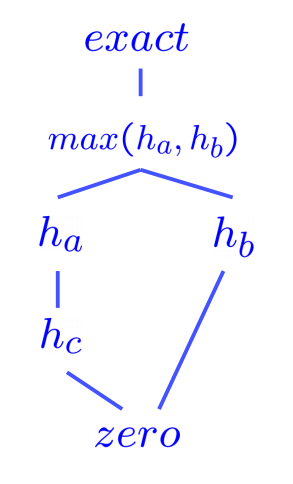
\includegraphics[height=6cm]{img/semi-lattice}
\end{center}
As a general rule, the $\max$ function applied to multiple admissible heuristics will also always be admissible. This is simply a consequence of all values output by the heuristics for any given state being constrained by the admissibility condition, $0 \leq h(n) \leq h^*(n)$. The maximum of numbers in this range must also fall in the same range. The same can be shown easily for multiple consistent heuristics as well. It's common practice to generate multiple admissible/consistent heuristics for any given search problem and compute the $\max$ over the values output by them to generate a heuristic that dominates (and hence is better than) all of them individually.

\end{document}